%%%%%%%%%%%%%%%%%%%%%%%%%%%%%%%%%%%%%%%%%%%%%%%%%%%%%%%%%%%%%%%%%%%%%%%%%%%%%%%
%%%%%%%%%%%%%%%%%%%%%%%%%%%%%%%%%%%%%%%%%%%%%%%%%%%%%%%%%%%%%%%%%%%%%%%%%%%%%%%
%%%%%%%%%%%%%%%%%%%%%%%%%%%%%%%%%%%%%%%%%%%%%%%%%%%%%%%%%%%%%%%%%%%%%%%%%%%%%%%
\chapter{Network Analysis}
\label{ch:appendix:analysis}
%%%%%%%%%%%%%%%%%%%%%%%%%%%%%%%%%%%%%%%%%%%%%%%%%%%%%%%%%%%%%%%%%%%%%%%%%%%%%%%
%%%%%%%%%%%%%%%%%%%%%%%%%%%%%%%%%%%%%%%%%%%%%%%%%%%%%%%%%%%%%%%%%%%%%%%%%%%%%%%
%%%%%%%%%%%%%%%%%%%%%%%%%%%%%%%%%%%%%%%%%%%%%%%%%%%%%%%%%%%%%%%%%%%%%%%%%%%%%%%
\begin{figure}[htb]
	\centering
	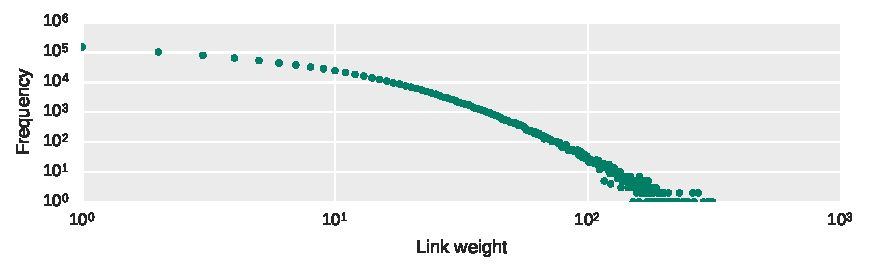
\includegraphics[width=\textwidth]{Figures/n123-edgeWeightDist}
	\caption[Link weight distribution for all snapshots]{\textbf{Link weight distribution for all snapshots}}
	\label{fig:123edges}
\end{figure}


\begin{figure}[htb]
	\centering
	\begin{subfigure}[b]{1.0\textwidth}
		\centering
		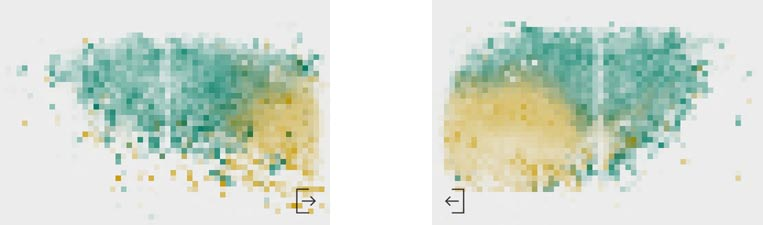
\includegraphics[width=\textwidth]{Figures/le_network1.pdf}
		\caption[Network 1]{Network 1}
		\label{fig:le1}
		\vspace*{5mm}
	\end{subfigure}
	%\vspace{1cm} 
	\begin{subfigure}[b]{1.0\textwidth}
		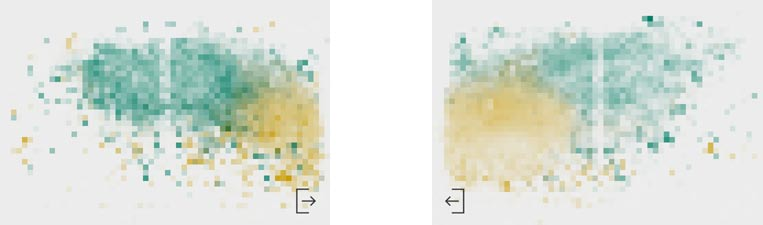
\includegraphics[width=\textwidth]{Figures/le_network2.pdf}
		\caption[Network 2]{Network 2}
		\label{fig:le2}
		\vspace*{5mm}
	\end{subfigure}
	%\vspace{1cm} 
	\begin{subfigure}[b]{1.0\textwidth}
		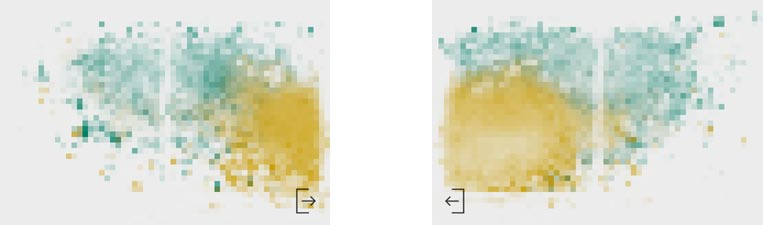
\includegraphics[width=\textwidth]{Figures/le_network3.pdf}
		\caption[Network 3]{Network 3}
		\label{fig:le3}
		\vspace*{5mm}
	\end{subfigure}
	\caption[Communities per network - leading eigenvector]{\textbf{Communities per network - leading eigenvector} The \emph{green} colour represents the younger community, containing the queen. The \emph{orange} color represents the older community. The hive exit on side A is on the bottom right and on side B on the bottom left. The data is aggredated for the complete timeframe of ten hours.}
	\label{fig:communitiesPerNetworkLE}
\end{figure}

\begin{figure}[htb]
	\centering
	\begin{subfigure}[b]{1.0\textwidth}
		\centering
		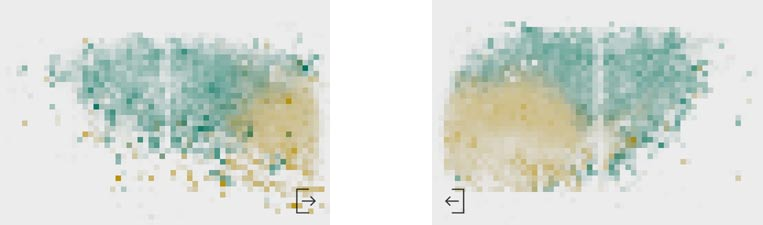
\includegraphics[width=\textwidth]{Figures/wt_network1.pdf}
		\caption[Network 1]{Network 1}
		\label{fig:wt1}
		\vspace*{5mm}
	\end{subfigure}
	%\vspace{1cm} 
	\begin{subfigure}[b]{1.0\textwidth}
		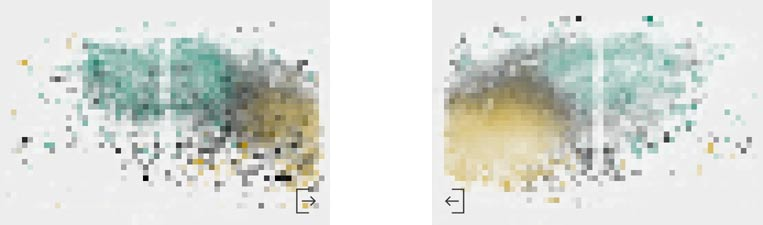
\includegraphics[width=\textwidth]{Figures/wt_network2.pdf}
		\caption[Network 2]{Network 2}
		\label{fig:wt2}
		\vspace*{5mm}
	\end{subfigure}
	%\vspace{1cm} 
	\begin{subfigure}[b]{1.0\textwidth}
		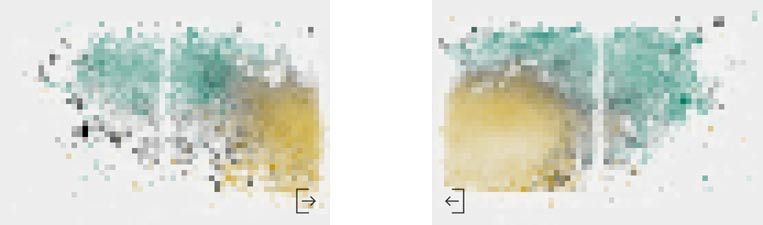
\includegraphics[width=\textwidth]{Figures/wt_network3.pdf}
		\caption[Network 3]{Network 3}
		\label{fig:wt3}
		\vspace*{5mm}
	\end{subfigure}
	\caption[Communities per network - walktrap]{\textbf{Communities per network - walktrap} The \emph{green} colour represents the younger community, containing the queen. The \emph{orange} color represents the older community. The \emph{gray} represents the middle-age community. The hive exit on side A is on the bottom right and on side B on the bottom left. The data is aggredated for the complete timeframe of ten hours.}
	\label{fig:communitiesPerNetworkWT}
\end{figure}



\begin{figure}[htb]
\centering
	\begin{subfigure}[b]{1.0\textwidth}
	\centering
	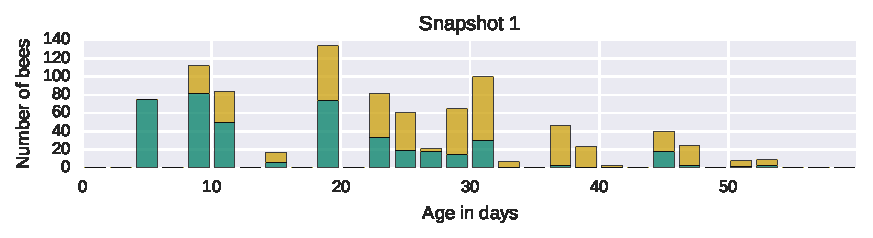
\includegraphics[width=1.0\textwidth]{Figures/n1-ageDistribution-LE}
	\end{subfigure}
	\begin{subfigure}[b]{1.0\textwidth}
	\centering
	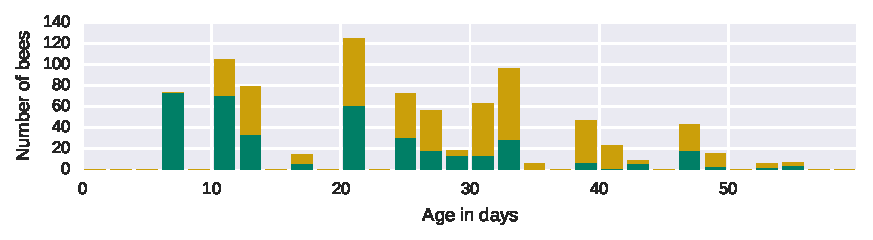
\includegraphics[width=1.0\textwidth]{Figures/n2-ageDistribution-LE}
	\end{subfigure}
	\begin{subfigure}[b]{1.0\textwidth}
	\centering
	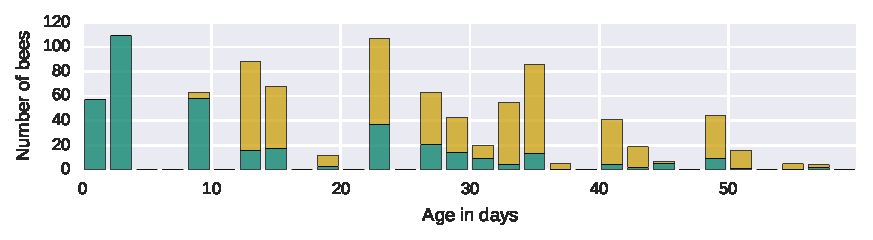
\includegraphics[width=1.0\textwidth]{Figures/n3-ageDistribution-LE}
	\end{subfigure}
	\caption[Age distribution for LE]{\textbf{Age distribution for LE}}
	\label{fig:ageDistLE}	
\end{figure}


\begin{figure}[htb]
\centering
	\begin{subfigure}[b]{1.0\textwidth}
	\centering
	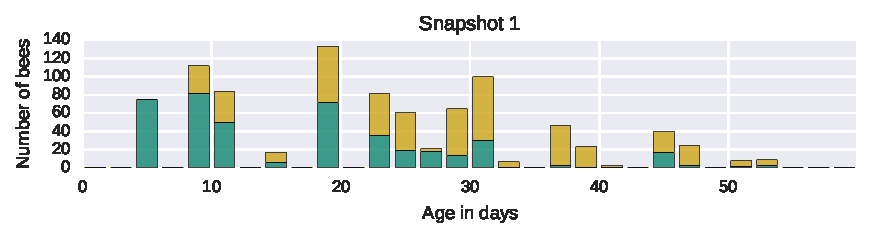
\includegraphics[width=1.0\textwidth]{Figures/n1-ageDistribution-WT}
	\end{subfigure}
	\begin{subfigure}[b]{1.0\textwidth}
	\centering
	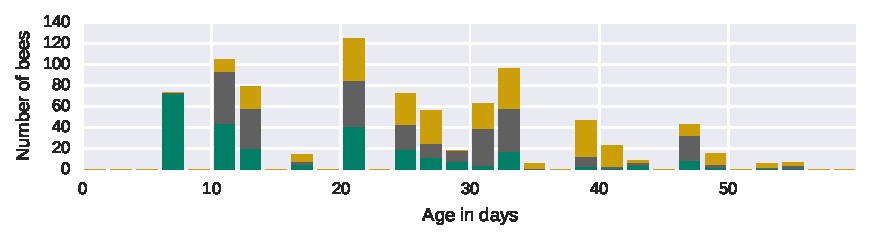
\includegraphics[width=1.0\textwidth]{Figures/n2-ageDistribution-WT}
	\end{subfigure}
	\begin{subfigure}[b]{1.0\textwidth}
	\centering
	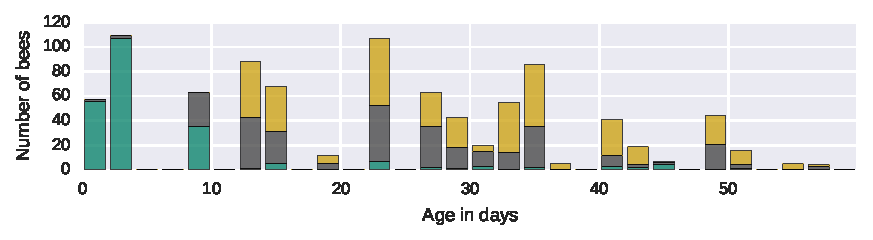
\includegraphics[width=1.0\textwidth]{Figures/n3-ageDistribution-WT}
	\end{subfigure}
	\caption[Age distribution per snapshot for WT]{\textbf{Age distribution per snapshot for WT}}
	\label{fig:ageDistWT}
\end{figure}


\begin{figure}[!h]
	\centering
	\begin{subfigure}[b]{1.0\textwidth}
	\centering
	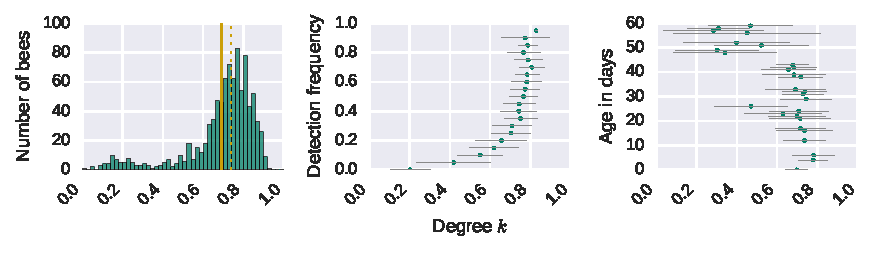
\includegraphics[width=1.0\textwidth]{Figures/n1-stat-degreeAgeDetF.pdf}
	%\caption[Degree]{\textbf{Degree}}
	%\label{fig:n3-degree}
	\end{subfigure}
	\begin{subfigure}[b]{1.0\textwidth}
	\centering
	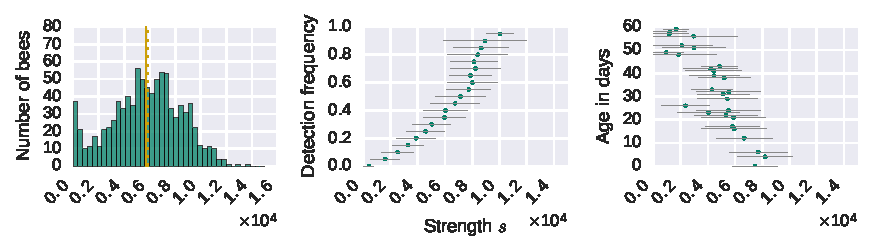
\includegraphics[width=1.0\textwidth]{Figures/n1-stat-strengthAgeDetF.pdf}
	%\caption[Strength]{\textbf{Strength}}
	%\label{fig:n3-strength}
	\end{subfigure}
	\begin{subfigure}[b]{1.0\textwidth}
	\centering
	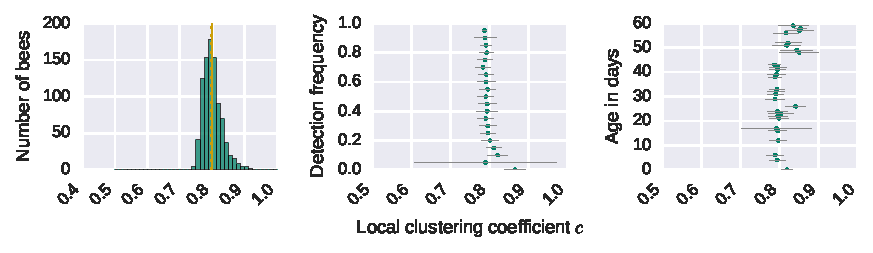
\includegraphics[width=1.0\textwidth]{Figures/n1-stat-lccAgeDetF.pdf}
	%\caption[Local clustering coefficient]{\textbf{Local clustering coefficient}}
	%\label{fig:n3-lcc}
	\end{subfigure}
	\begin{subfigure}[b]{1.0\textwidth}
	\centering
	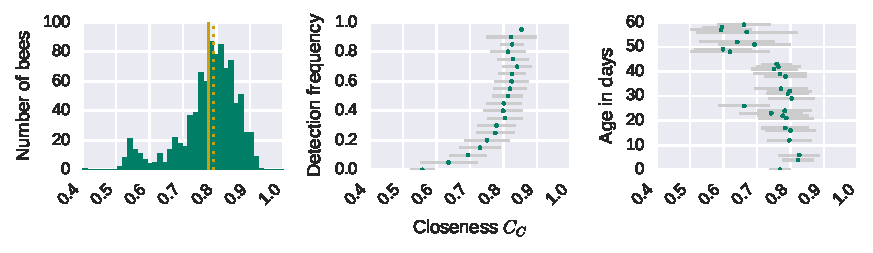
\includegraphics[width=1.0\textwidth]{Figures/n1-stat-closenessAgeDetF.pdf}
	%\caption[Closeness Centrality]{\textbf{Closeness Centrality}}
	%\label{fig:n3-closeness}
	\end{subfigure}
	\begin{subfigure}[b]{1.0\textwidth}
	\centering
	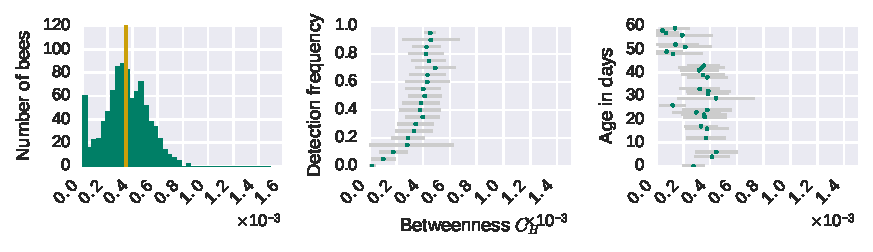
\includegraphics[width=1.0\textwidth]{Figures/n1-stat-betweenAgeDetF.pdf}
	%\caption[Betweeness Centrality]{\textbf{Betweeness Centrality}}
	%\label{fig:n3-between}
	\end{subfigure}
	\caption[Snapshot 1: Local measures in relation to age and detection frequency]{\textbf{Snapshot 1: Local measures in relation to age and detection frequency}}
	\label{fig:n1-degreeStrLCC}
\end{figure}

\begin{figure}[!h]
	\centering
	\begin{subfigure}[b]{1.0\textwidth}
	\centering
	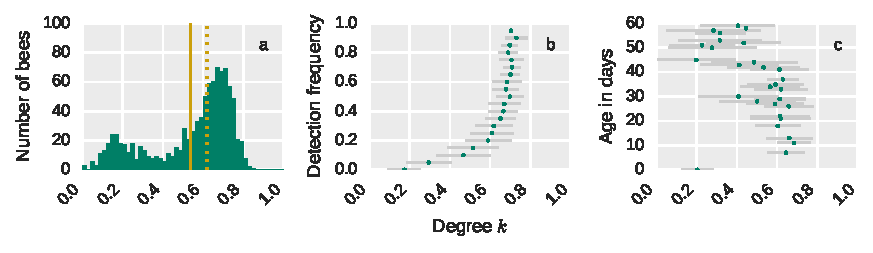
\includegraphics[width=1.0\textwidth]{Figures/n2-stat-degreeAgeDetF.pdf}
	%\caption[Degree]{\textbf{Degree}}
	%\label{fig:n3-degree}
	\end{subfigure}
	\begin{subfigure}[b]{1.0\textwidth}
	\centering
	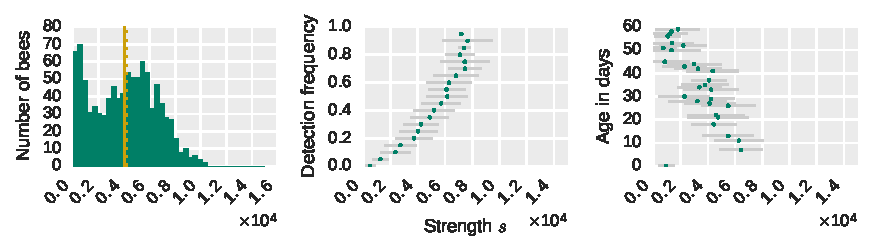
\includegraphics[width=1.0\textwidth]{Figures/n2-stat-strengthAgeDetF.pdf}
	%\caption[Strength]{\textbf{Strength}}
	%\label{fig:n3-strength}
	\end{subfigure}
	\begin{subfigure}[b]{1.0\textwidth}
	\centering
	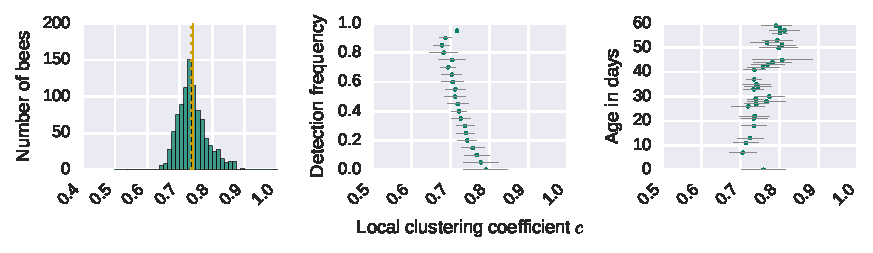
\includegraphics[width=1.0\textwidth]{Figures/n2-stat-lccAgeDetF.pdf}
	%\caption[Local clustering coefficient]{\textbf{Local clustering coefficient}}
	%\label{fig:n3-lcc}
	\end{subfigure}
	\begin{subfigure}[b]{1.0\textwidth}
	\centering
	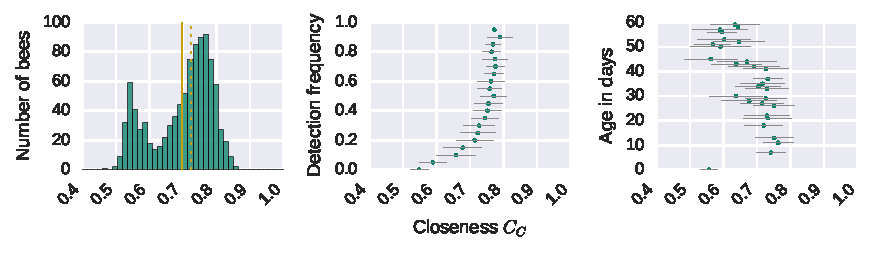
\includegraphics[width=1.0\textwidth]{Figures/n2-stat-closenessAgeDetF.pdf}
	%\caption[Closeness Centrality]{\textbf{Closeness Centrality}}
	%\label{fig:n3-closeness}
	\end{subfigure}
	\begin{subfigure}[b]{1.0\textwidth}
	\centering
	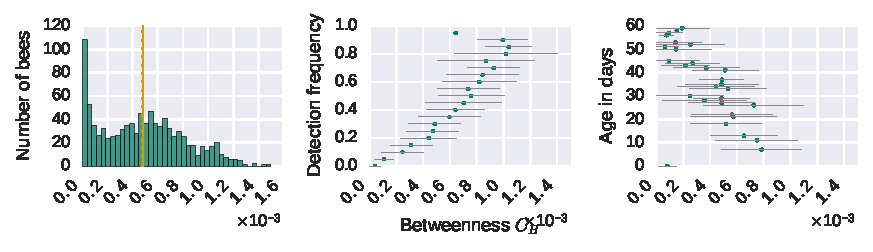
\includegraphics[width=1.0\textwidth]{Figures/n2-stat-betweenAgeDetF.pdf}
	%\caption[Betweeness Centrality]{\textbf{Betweeness Centrality}}
	%\label{fig:n3-between}
	\end{subfigure}
	\caption[Snapshot 2: Local measures in relation to age and detection frequency]{\textbf{Snapshot 2: Local measures in relation to age and detection frequency}}
	\label{fig:n2-degreeStrLCC}
\end{figure}

\begin{figure}
	\centering
	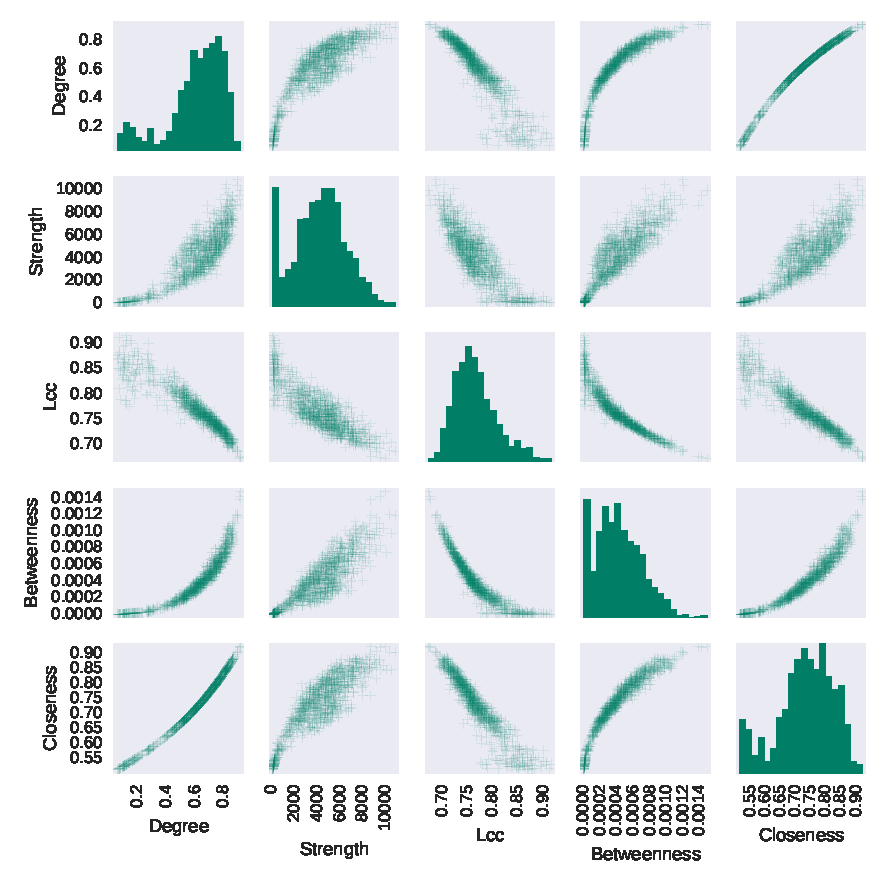
\includegraphics[width=1.0\textwidth]{Figures/n3_scatter}
	\caption[Scatter plot for node level measure]{\textbf{Scatter plot for node level measure}}
	\label{fig:n3:scatter}
\end{figure}


\begin{figure}[htb]
\centering
	\begin{subfigure}[b]{1.0\textwidth}
	\centering
	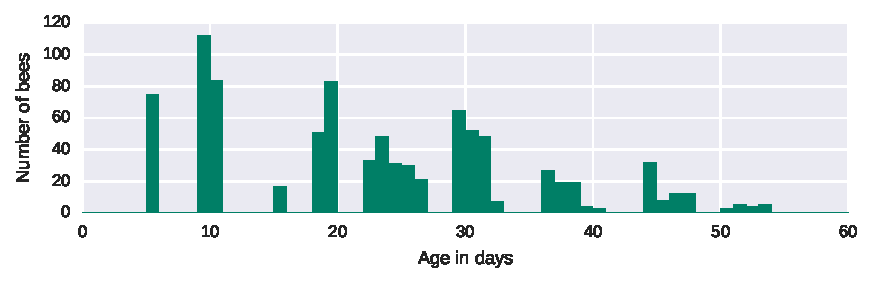
\includegraphics[width=1.0\textwidth]{Figures/n1_ages}
	\end{subfigure}
	\begin{subfigure}[b]{1.0\textwidth}
	\centering
	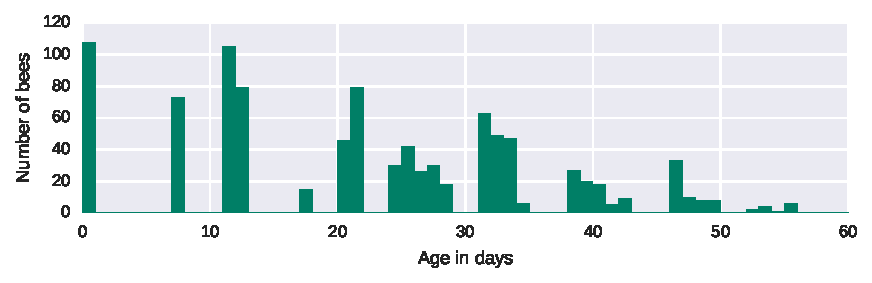
\includegraphics[width=1.0\textwidth]{Figures/n2_ages}
	\end{subfigure}
	\begin{subfigure}[b]{1.0\textwidth}
	\centering
	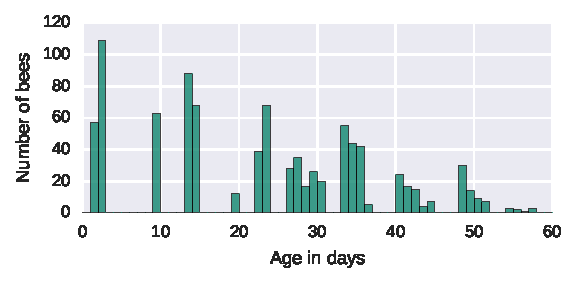
\includegraphics[width=1.0\textwidth]{Figures/n3_ages}
	\end{subfigure}
	\caption[Age distribution per snapshot]{\textbf{Age distribution per snapshot}}
	\label{fig:agesAll}	
\end{figure}